\section{Equilibrium \& Comparative Statics}
\label{sec:section3} 
\subsection{Steady State Equilibrium and Computation}\label{sec:section3.1} 
Using the framework and results above, I now present a refined definition for the steady state equilibrium of the market: 
\begin{definition}
    A Steady State Equilibrium (SSE) is a triplet $(\mu^*, \omega^*, \Psi^*)$ such that:
    \begin{enumerate}
        \item $ \mu^*(\theta,b) \text{ attains } V_m(\theta,b), \; \forall\, \theta, b \in \Theta \times \mathcal{B}_m$, given $\omega^*,\Psi^*$
        \item $ \omega^*(\theta,b) \text{ attains } V_w(\theta,b), \; \forall\, \theta, b \in \Theta \times \mathcal{B}_w$, given $\mu^*,\Psi^*$
        \item $\Psi^*$ satisfies Equations \ref{eq:ss1}, \ref{eq:ss2}, and \ref{eq:ss3} given the strategy profile $(\mu^*, \omega^*)$
    \end{enumerate} 
\end{definition}

Intuitively, the above definition establishes two requirements that must be satisfied by an equilibrium market configuration. 
Firstly, it must be the case that $\mu^*$ and $\omega^*$ are mutual best responses given the platform state $\Psi^*$ for which, as previously outlined, a necessary and sufficient condition would have them each solve the sex-specific MDP. 
These two conditions alone correspond to \textit{partially rational expectations equilibria} (PREE), as per \cite{burdett1997marriage}, since they require agents to play optimally for some fixed steady state $\Psi^*$, imposing rationality on all game aspects other than the platform state dynamics.  
Furthermore, in line with mean-field game theory literature, a \textit{consistency check} is imposed by the third condition, which requires that the platform steady state to which agents are best-responding with $(\mu^*,\omega^*)$ is sustained as a fixed point, thus constraining the set of PREE to define full steady state equilibria. 

Although formal proofs for the existence and uniqueness of steady-state equilibria are outside the scope of this paper, I rely on numerical procedures\footnote{The code required to reproduce all presented analysis is accessible under the GitHub repository \texttt{patohdzs/project-swipe}, with most dependencies covered by the SciPy Stack packages.} to approximate equilibria under various exogenous settings. This approach has been frequently employed by related works \citep[see][]{iyer2014mean, gummadi2011optimal} as it can help uncover insights provided by mean-field models. To compute model equilibria, I frame the recurrence relation presented in \autoref{prop:recurrence relation}, as well as Equations \ref{eq:ss1}, \ref{eq:ss2}, and \ref{eq:ss3}, as a system of $2(|\mathcal{B}_m|+|\mathcal{B}_w|+1)$ non-linear equations, and solve this using a modified version of the hybrid Powell method, as implemented by the MINPACK 1 routine \citep{more1980user}  

\subsection{Best Response Analysis}\label{sec:section3.2} 
Using the computational procedures outlined above, a number of insights can be uncovered related to how exogenous parameters affect an agent's best-response swiping strategy. The first parameter I analyse is the discount factor, which represents the probability of remaining inside the platform for an additional time period, but is often interpreted as the representative agent's patience level. To determine the effects of changes in the discount factor, I computed the best-response policy over a range of different values for $\delta$ (using an arbitrary set of exogenous parameters), with results shown in \autoref{fig:discount-cs}. Evidently, as the agent becomes less patient, they `lower their standards' for potential matches in the platform, shifting their swiping curve downwards. 

\begin{figure}[ht] 
    \centering
    \caption{Comparative Statics on the Discount Factor}
    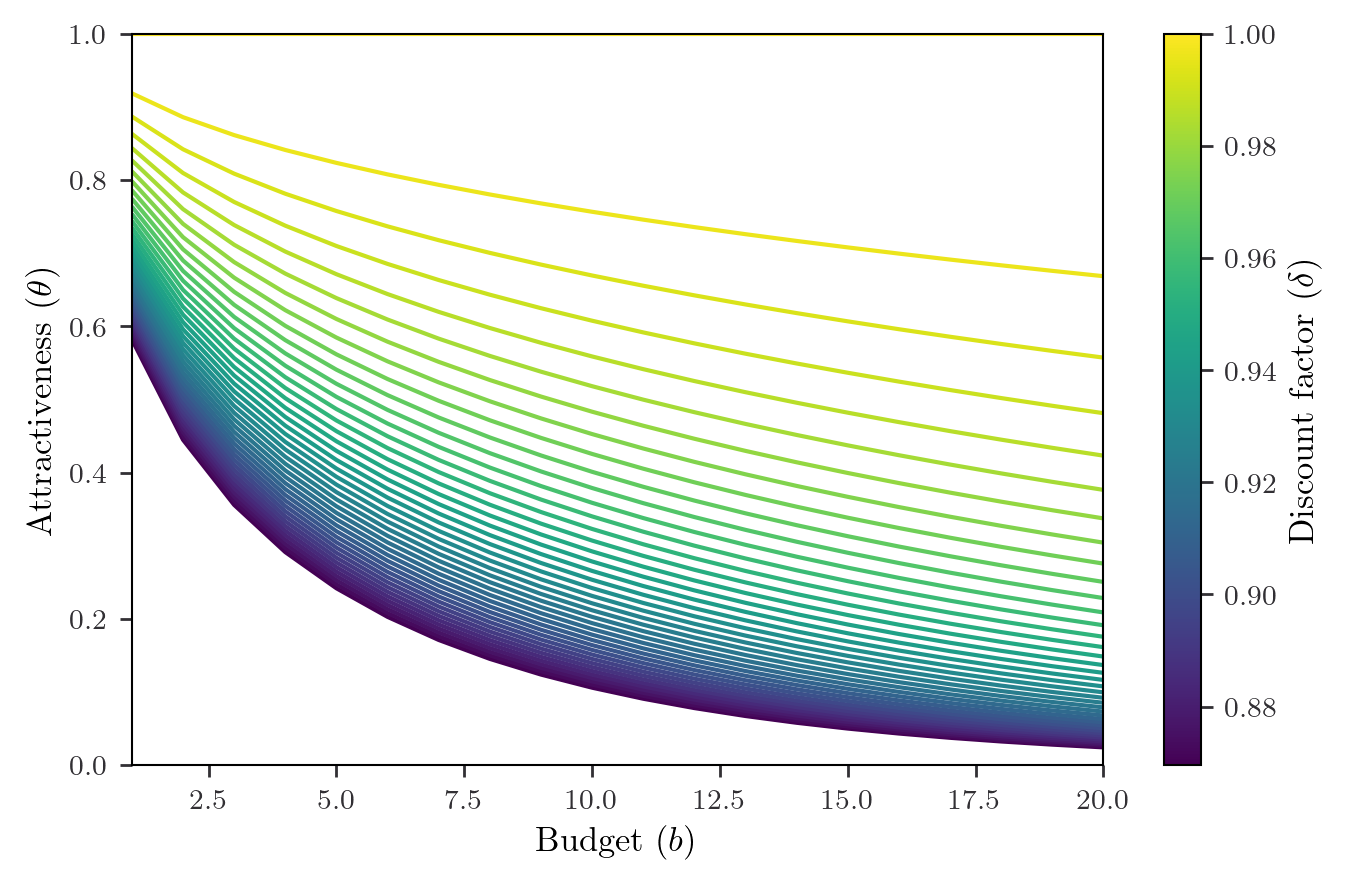
\includegraphics{discount-cs.png}
    \label{fig:discount-cs}
\end{figure} 

Another interesting parameter to examine is the absolute risk aversion of agents, which I choose to interpret as their `desperateness' for matching. In the platform, risk-averse agents prefer a higher chance of matching (even if these yield relatively lower payoffs), whilst risk-loving agents prefer to wait around and save their swipes for high-yield candidates. To perform comparative statics on this parameter, I fix a CARA utility function for agents, with parameter $r$ corresponding to the Arrow-Pratt coefficient for absolute risk aversion. I then compute the optimal swiping rule for various different values of $r$, with results for this shown on \autoref{fig:risk-cs}. From here, it is evident that as agents become `more desperate' for matches, implied by rising absolute risk aversion, they lower their standards for right-swiping on a candidate, thus shifting their swiping curve downwards.

\begin{figure}[ht]
    \centering
    \caption{Comparative Statics on Absolute Risk Aversion}
    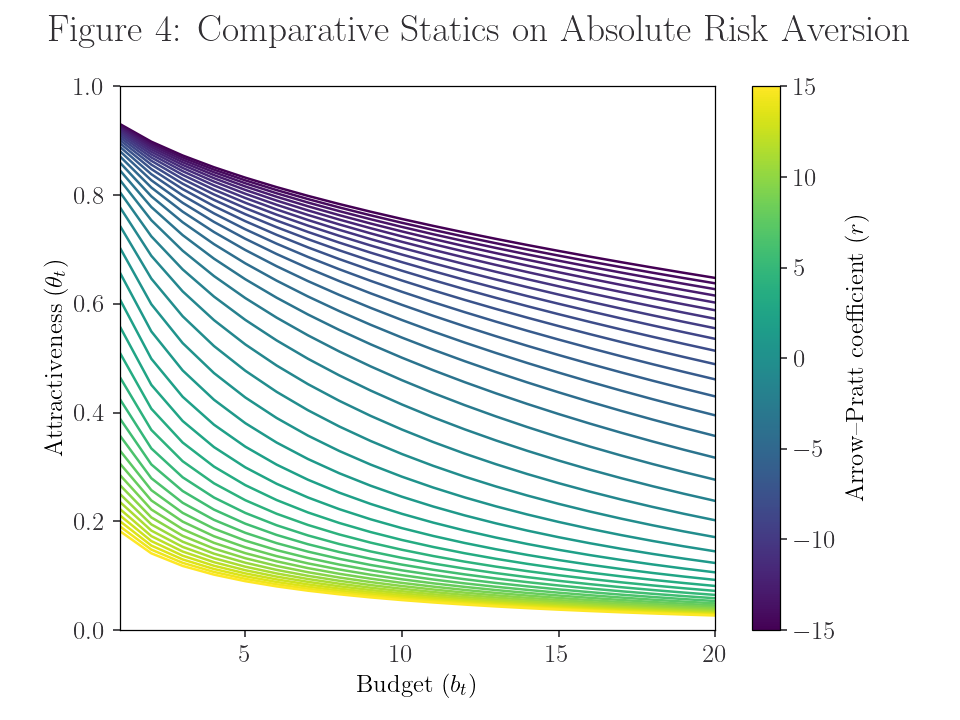
\includegraphics{risk-cs.png}
    \label{fig:risk-cs} 
\end{figure}

\subsection{Market Configuration Analysis}\label{sec:section3.3} 
Finally, I perform comparative statics at the platform level to determine how different factors affect market configurations. This is especially important as it considers not only the effects on best-responses for one sex, but also how these propagate across the market through its aggregate state. More specifically, I focus the aforementioned `Fast-Swiping Males' puzzle, investigating the discrepancies in swiping rates and matching outcomes between men and women, and I present a possible explanation for which the above model can replicate these outcomes. 
% Both of these explanations attribute this phenomenon to gender imbalances within the platform (which estimates place between a 2:1 and a 10:1 male-to-female ratio), but, crucially, the way this imbalance arises can change other platform aspects significantly in equilibrium. 
%The first of these involves differences in attractiveness between men and women, a conjecture motivated by research undertaken by OkCupid, which shows

Fundamentally, the main scenario that could induce the `Fast-Swiping Males' puzzle involves differential arrival flows between men and women, which occur exogenously within my model but are in line with empirical findings, which place. To asses the market configurations arising from of this situation, I compute the model equilibria under a 6:1 ratio between arrival rates $\lambda_m$ and $\lambda_w$. The results for this are shown in \autoref{fig:mkt-cs}, highlighting three main insights for this scenario. 

\begin{figure}[ht]
    \centering
    \caption{Market Configuration Under Differential Agent Inflows}
    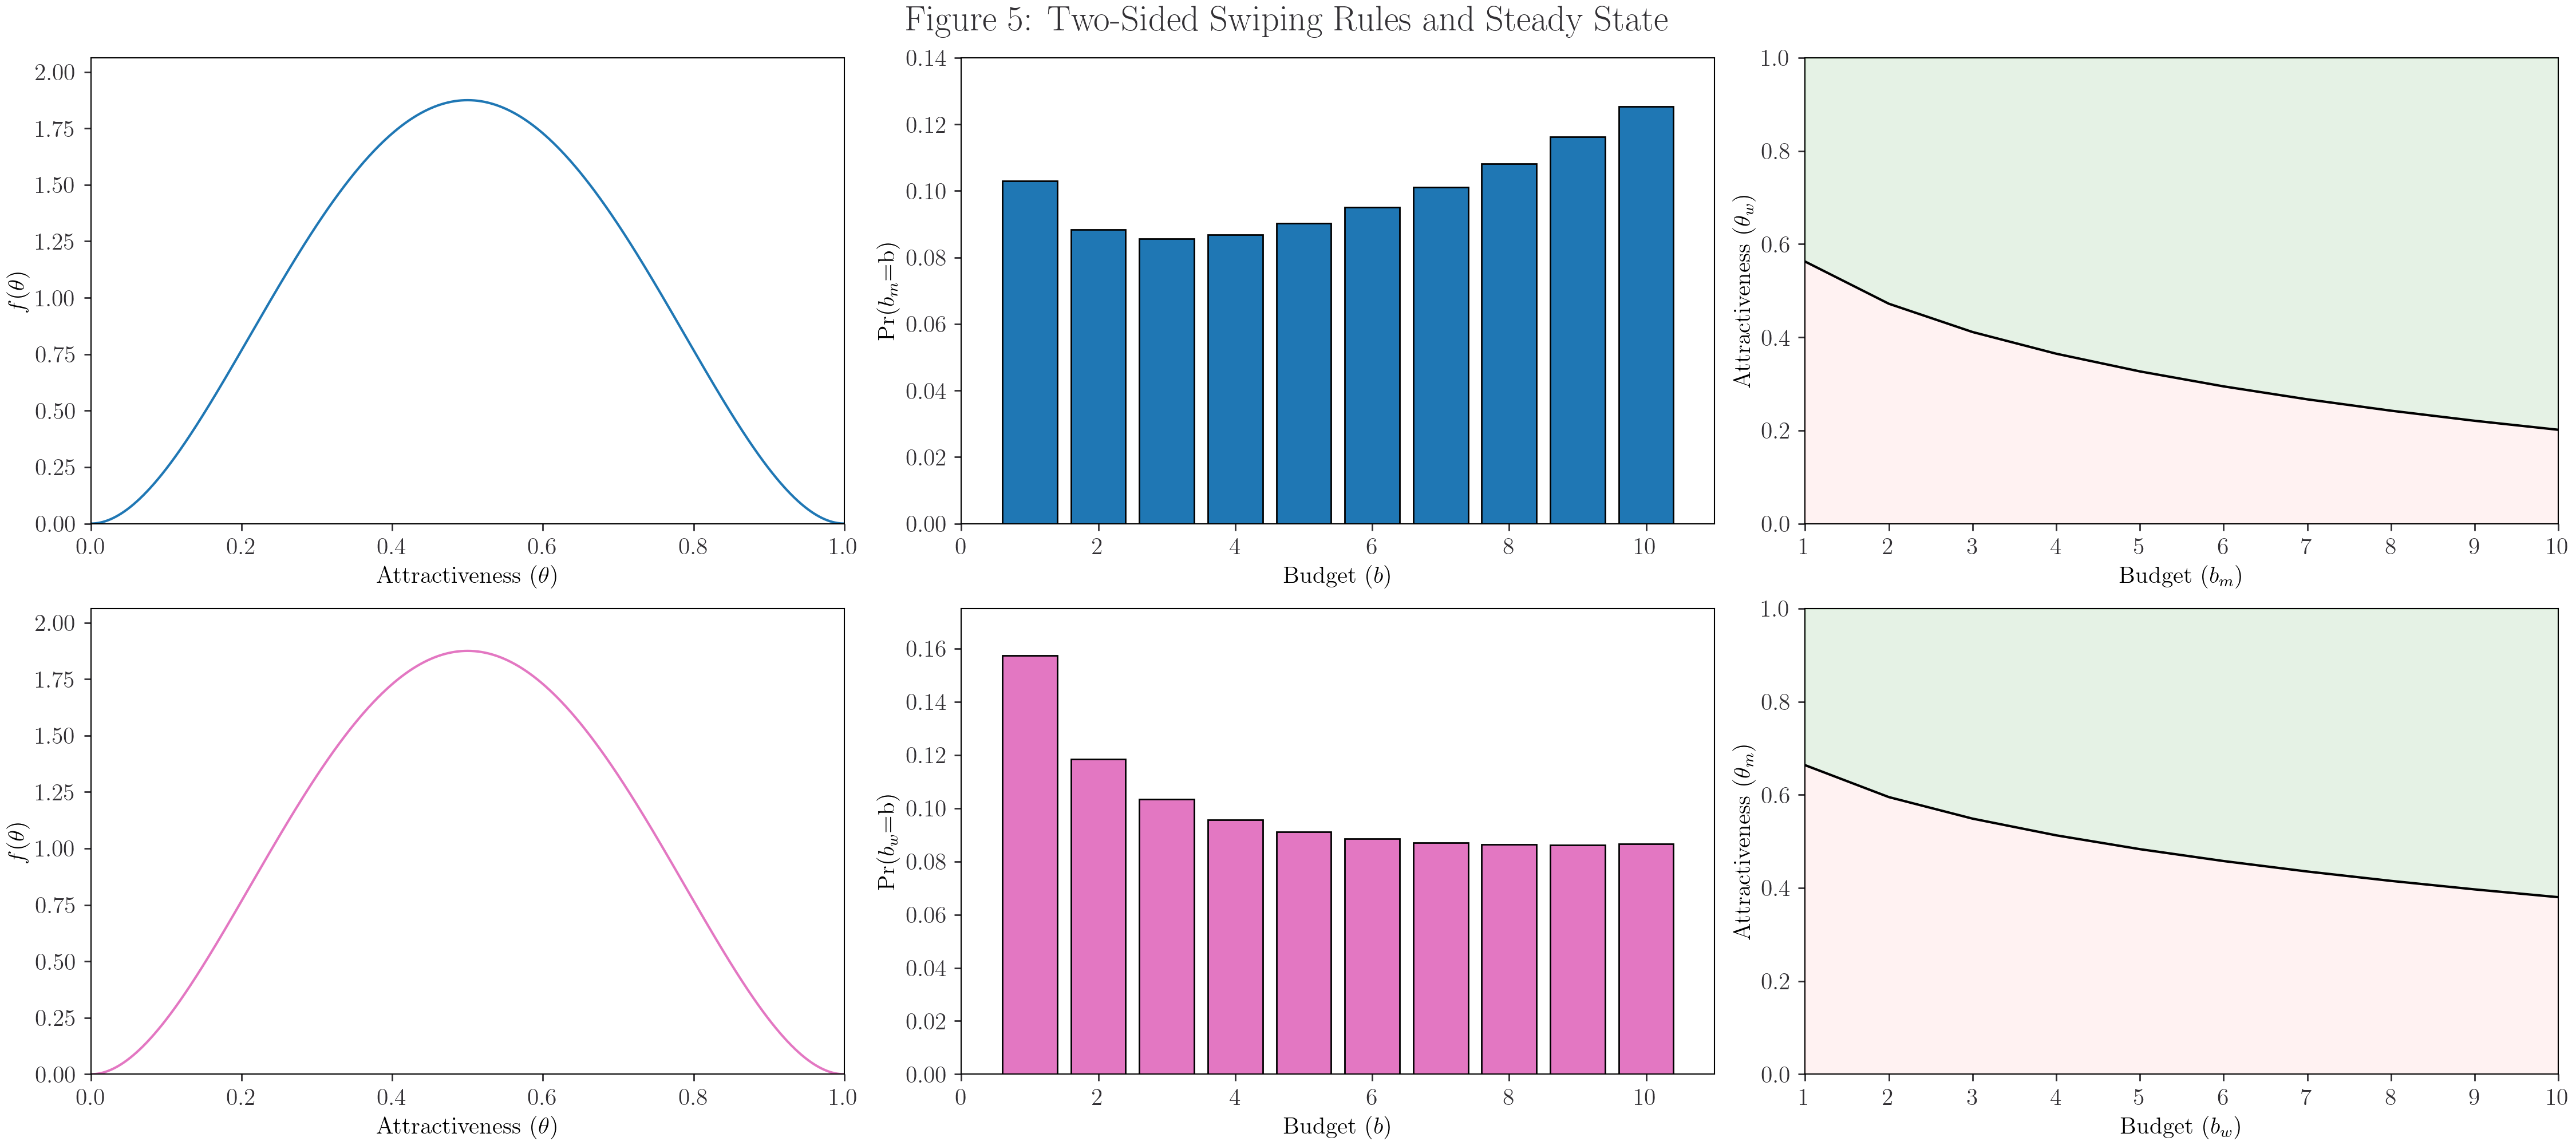
\includegraphics{mkt-cs.png}
    \label{fig:mkt-cs} 
\end{figure} 

Firstly, under the above scenario, the steady-state mass of male agents in the platform is around ten times greater than that of female agents (in line with empirical estimates), implying that male agents face a tight market and struggle to get paired with female candidates. This is further evidenced by the top-center plot within \autoref{fig:mkt-cs}, which shows that male agents are highly concentrated in the top budget levels. Due to the effect of market tightness on the effective discount rate, male agents are also more impatient than women on the platform, which makes sense intuitively as they also face considerably worse matching odds. This effect is captured by their best-response strategy, which sits considerably lower than the female swiping curve, effectively showing how a congested market lowers male patience and by extension, their standards, leading them to swipe right on most women. Ultimately, this explains the `Fast-Swiping Males' puzzle given that, under this particular equilibrium, men receive right-swipes with probability $\overline\omega=0.491$, compared to $\overline\mu=0.988$ for women, thus replicating the observed phenomenon through a traceable shock on agent inflows.